

\section{Additional NS Examples}
\label{appendix:MoreNsExamples}


%\subsection{Motivating Examples --- Explanation}
%
%
%Observe the simple program depicted in Listing~\ref{lst:MotivatingExample1Ser}. Each  {\color{ForestGreen}$\blacklozenge_\text{main}$} gives rise to a fresh in-flight request. The variable ``X'' is global, and shared among all in-flight requests, while the variable ``y'' is a local variable, per each request. 
%%
%As there are no yields, it is straightforward to see that the program is trivially serializable, with every request {\color{ForestGreen}$\blacklozenge_\text{main}$}: (i) assigning 1 to the global variable X; (ii) assigning y the value of X, i.e., always 1; (iii) assigning X the value 0; and (iv) returning the response y ({\color{red}$\blacklozenge_1$}). This results to every request/response pair to be of the form {\color{ForestGreen}$\blacklozenge_\text{main}$}/{\color{red}$\blacklozenge_1$}.
%%
%The program is slightly altered (in Listing~\ref{lst:MotivatingExample2NonSer}), by adding a yield operation between the aforementioned steps (i) and (ii). Now, by running two {\color{ForestGreen}$\blacklozenge_\text{main}$} requests that interleave, it is possible to attain a {\color{ForestGreen}$\blacklozenge_\text{main}$}/{\color{red}$\blacklozenge_0$} request/response pair, which is unattainable in any serial execution of Listing~\ref{lst:MotivatingExample2NonSer} --- as any such serial execution is equivalent to Listing~\ref{lst:MotivatingExample1Ser}, which always responds {\color{red}$\blacklozenge_1$} to any request {\color{ForestGreen}$\blacklozenge_\text{main}$}.
%%
%The program is altered once again in in Listing~\ref{lst:MotivatingExample3Ser}, by adding a fresh global variable ``L'', indicating whether the critical section is locked ($L=1$) or not ($L=0$).
%By adding a global lock variable, even if an interleaving occurs after yielding, the lock will allow only the first request to terminate, and will then release the lock for the next request. Hence, despite having yields, we attain serializable executions, and only {\color{ForestGreen}$\blacklozenge_\text{main}$}/{\color{red}$\blacklozenge_1$} request/response pairs are produced, similar to the original program in Listing~\ref{lst:MotivatingExample1Ser}.
%%
%This simple example demonstrates the motivation for automatic serializability checking, as even small, toy programs can be surprisingly difficult to reason about when assessing their serializable behavior.
%





\subsection{Motivating Example \#1}
\label{appendix:subsec::Ex1A:NS}


For our first motivating example, presented in Listing~\ref{lst:MotivatingExample1Ser}, we present the Network System in Fig.~\ref{fig:code1ExampleNS}, the Serialized NFA in Fig.~\ref{fig:code1ExampleNFA}, and the Interleaving Petri Net in Fig.~\ref{fig:code1ExamplePN}.


%\begin{minipage}[t]{0.3\textwidth}
%	\begin{lstlisting}[caption={Without yield or lock (serializable)}]
%	request main: 
%		X := 1 
%		// no yield
%		y := X 
%		X := 0
%		return y 
%	\end{lstlisting}
%\end{minipage}

\begin{figure}[!htbp]
	\centering
	% \includegraphics[width=\textwidth]{plots/code_single_path_NS.png}\\[1ex]
	
	\begin{tikzpicture}[
		node distance=1.5cm and 2.5cm,
		>=stealth,
		thick,
		every node/.style={font=\small}
		]
		%––– Request (main) –––
		\node[
		draw=black,
		line width=0.8pt,
		fill=ForestGreen!20,
		text=black,
		diamond,
		aspect=2,
		inner sep=2pt,
		scale=0.7
		] (main) {\texttt{main}};
		
		%––– First state: y=0 + full program –––
		\node[right=0.7cm of main, align=center] (state1) {
			\begin{tikzpicture}[baseline=(ybox.base)]
				\node[
				draw=black,
				line width=0.8pt,
				fill=brightyellow,
				text=black,
				rectangle,
				rounded corners=1pt,
				inner sep=2pt
				] (ybox) {\texttt{y=0}};
			\end{tikzpicture}\\[-2.5pt]
			\begin{minipage}{2cm}
				\begin{lstlisting}[language=CustomPseudoCode,numbers=none,basicstyle=\tiny\ttfamily]
X := 1
// no yield
y := X
X := 0
return y
				\end{lstlisting}
			\end{minipage}
		};
		
		%––– Second state: y=1 + //end –––
		\node[right=of state1, align=center] (state2) {
			\begin{tikzpicture}[baseline=(ybox.base)]
				\node[
				draw=black,
				line width=0.8pt,
				fill=brightyellow,
				text=black,
				rectangle,
				rounded corners=1pt,
				inner sep=2pt
				] (ybox) {\texttt{y=1}};
			\end{tikzpicture}\\[-2.5pt]
			\begin{minipage}{0.8cm}
				\begin{lstlisting}[language=CustomPseudoCode,numbers=none,basicstyle=\tiny\ttfamily]
// end
				\end{lstlisting}
			\end{minipage}
		};
		
		%––– Response "1" –––
		\node[
		right=0.6cm of state2,
		draw=black,
		line width=0.8pt,
		fill=RedViolet!20,
		text=black,
		diamond,
		aspect=2,
		inner sep=2pt,
		scale=0.7,
		font=\Large
		] (resp1) {\texttt{1}};
		
		%––– Arrows –––
		\draw[->] (main) -- (state1);
		
		% Single transition label: X=0 -> X=1
		\draw[->] (state1) -- node[above] {%
			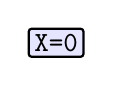
\begin{tikzpicture}[baseline=(a.base)]
				\node[draw=black,line width=0.8pt,fill=blue!10,rectangle,rounded corners=1pt,inner sep=2pt] (a) {\texttt{X=0}};
			\end{tikzpicture}
			$\to$
			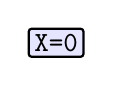
\begin{tikzpicture}[baseline=(b.base)]
				\node[draw=black,line width=0.8pt,fill=blue!10,rectangle,rounded corners=1pt,inner sep=2pt] (b) {\texttt{X=0}};
			\end{tikzpicture}
		} (state2);
		
		% To response "1"
		\draw[->] (state2) -- (resp1);
		
	\end{tikzpicture}
	
	\caption{Network System for interleaving executions of the program in Listing~\ref{lst:MotivatingExample1Ser}.}
\label{fig:code1ExampleNS}
\end{figure}



%\begin{figure}[!htbp]
%	\centering
%	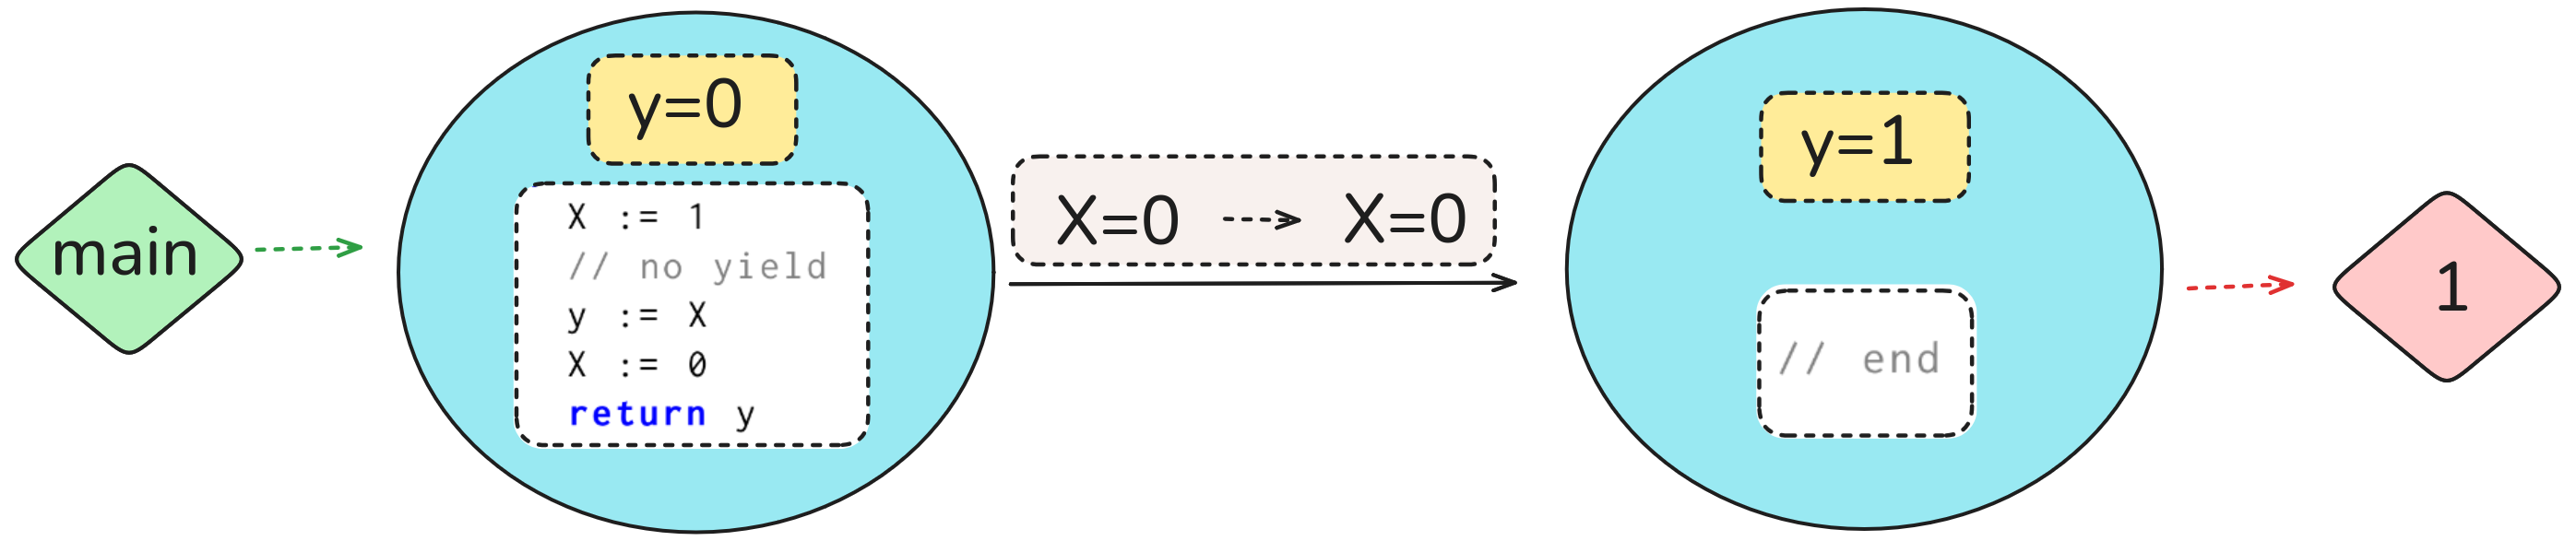
\includegraphics[width=0.9\textwidth]{plots/code_1_NS.png}
%	\caption{Network System for interleaving executions of the program in Listing~\ref{lst:MotivatingExample1Ser}.}
%	\label{fig:code1ExampleNS}
%\end{figure}


%\begin{figure}[!htbp]
%	\centering
%	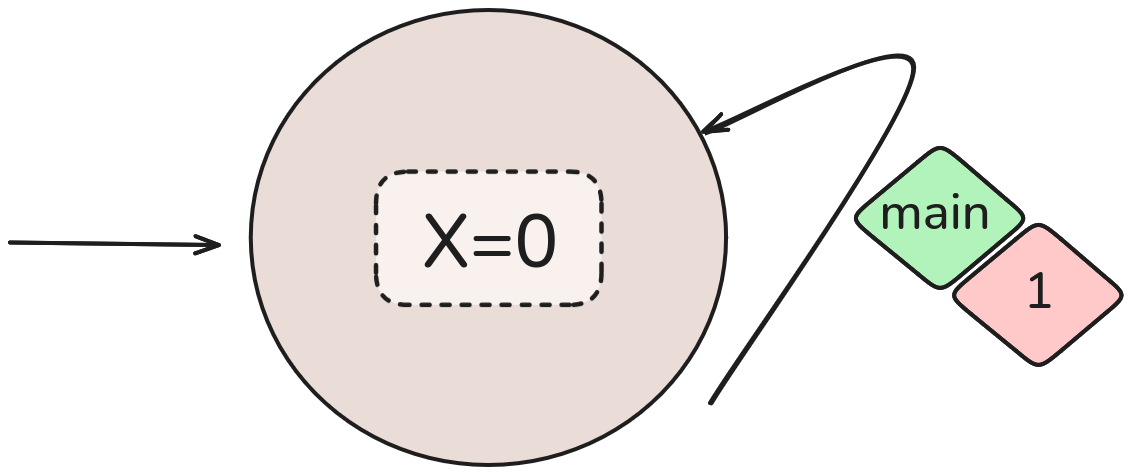
\includegraphics[width=0.35\textwidth]{plots/code_1_NFA.png}
%	\caption{NFA for serial executions of the program in Listing~\ref{lst:MotivatingExample1Ser}.}
%	\label{fig:code1ExampleNFA}
%\end{figure}


\begin{figure}  [!htbp]
	\centering
	% \includegraphics[width=0.48\textwidth,trim=0 0 0 0,clip]{plots/code_single_X0_NFA.pdf}
	
	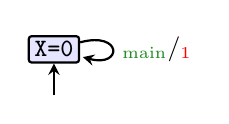
\begin{tikzpicture}[
		->,>=stealth,
		thick,
		node distance=2.5cm,
		state/.style={
			draw=black,
			line width=0.8pt,
			fill=blue!10,
			rectangle,
			rounded corners=1pt,
			inner sep=2pt,
			font=\small
		},
		every node/.style={font=\small}
		]
		% Single state
		\node[state] (X0) {\texttt{X=0}};
		
		% Initial state arrow
		\draw[->] ([yshift=-0.4cm]X0.south) -- (X0.south);
		
		% Self-loop with main/1 using the paper's colored lozenge notation
		\draw[->] (X0) edge[loop right]
		node[right] {${\color{ForestGreen}\blacklozenge_{\mathrm{main}}}/{\color{red}\blacklozenge_1}$} (X0);
	\end{tikzpicture}
	
	\caption{NFA for serial executions of the program in Listing~\ref{lst:MotivatingExample1Ser}.}
\label{fig:code1ExampleNFA}
\end{figure}




\begin{figure}[H]
	\centering
	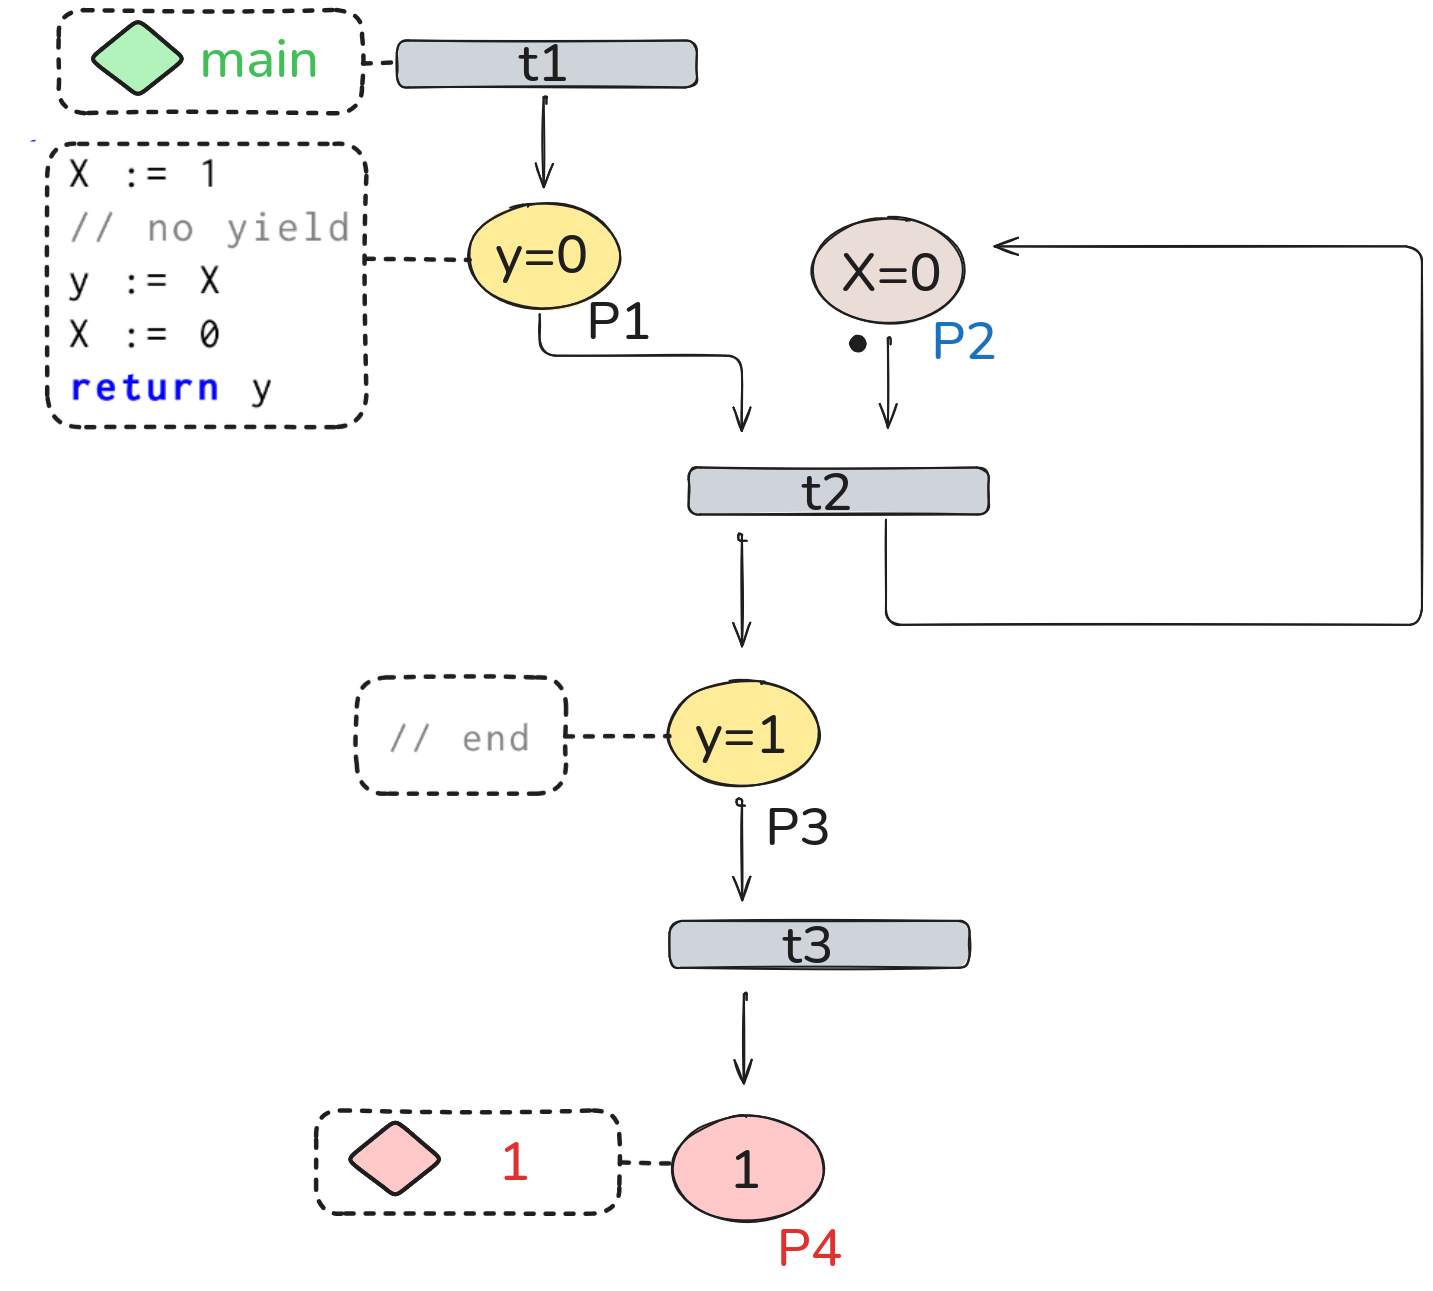
\includegraphics[width=0.6\textwidth]{plots/code_1_PN_with_annotation.png}
	\caption{Petri Net for interleaving executions of the program in Listing~\ref{lst:MotivatingExample1Ser}.}
	\label{fig:code1ExamplePN}
\end{figure}


%

\subsection{Motivating Examples \#2}
\label{appendix:subsec::Ex1B:NS}

For details, see the main text (Sec.~\ref{sec:problem-definition}).


\subsection{Motivating Examples \#3}
\label{appendix:subsec:Ex1C:NS}


For our third motivating example, presented in Listing~\ref{lst:MotivatingExample3Ser}, we present the Network System in Fig.~\ref{fig:code3ExampleNS}, the Serialized NFA in Fig.~\ref{fig:code3ExampleNFA}, and the Interleaving Petri Net in Fig.~\ref{fig:code3ExamplePN}

%\begin{minipage}[t]{0.3\textwidth}
%	\begin{lstlisting}[caption={With yield and lock (serializable)}]
%		request foo: 
%			// lock
%			while (L == 1): 
%				yield
%			L := 1 
%		
%			X := 1
%			yield
%			y := X 
%			X := 0
%		
%			// unlock    
%			L := 0
%			return y 
%	\end{lstlisting}
%\end{minipage}
%
%This program corresponds to the following Network System (NS):

%\begin{figure}[!htbp]
%	\centering
%	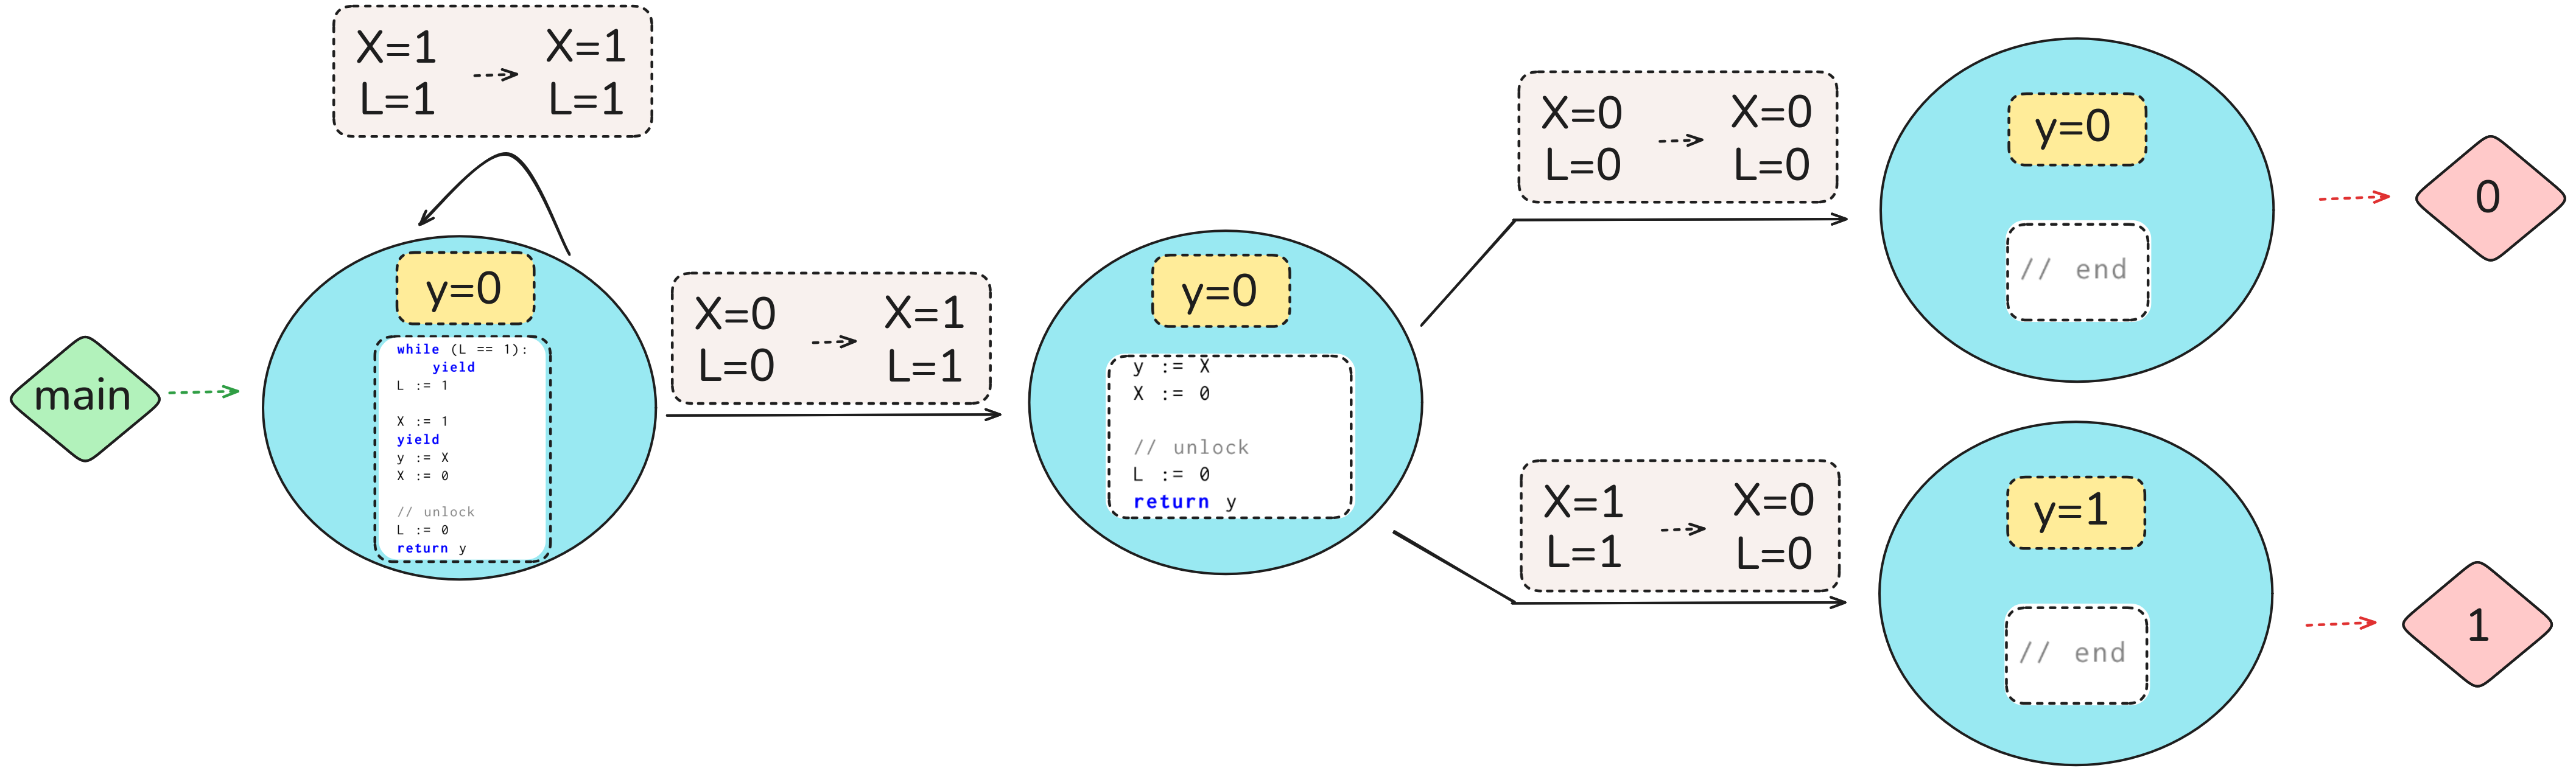
\includegraphics[width=1.1\textwidth]{plots/code_3_NS.png}
%	\caption{Network System for interleaving executions of the program in Listing~\ref{lst:MotivatingExample3Ser}.}
%	\label{fig:code3ExampleNS}
%\end{figure}


\begin{figure}[!htbp]
	\centering
	% \includegraphics[width=\textwidth]{plots/code_locking_NS.png}\\[1ex]
	
	\begin{tikzpicture}[
		node distance=1.5cm and 2.5cm,
		>=stealth,
		thick,
		every node/.style={font=\small}
		]
		%–––– Request (green diamond) ––––
		\node[
		draw=black,
		line width=0.8pt,
		fill=ForestGreen!20,
		text=black,
		diamond,
		aspect=2,
		inner sep=2pt,
		scale=0.7
		] (main) {\texttt{main}};
		
		%–––– State 1: y=0 + locked program ––––
		\node[right=0.7cm of main, align=center] (state1) {
			\begin{tikzpicture}[baseline=(ybox.base)]
				\node[
				draw=black,
				line width=0.8pt,
				fill=brightyellow,
				text=black,
				rectangle,
				rounded corners=1pt,
				inner sep=2pt
				] (ybox) {\texttt{y=0}};
			\end{tikzpicture}\\[-2.5pt]
			\begin{minipage}{2.6cm}
				\begin{lstlisting}[language=CustomPseudoCode,numbers=none,basicstyle=\tiny\ttfamily]
while (L == 1):
	yield
L := 1

X := 1
yield
y := X
X := 0

// unlock
L := 0
return y
				\end{lstlisting}
			\end{minipage}
		};
		
		%–––– State 2: y=0 + tail program ––––
		\node[right=of state1, xshift=12mm, align=center] (state2) {
			\begin{tikzpicture}[baseline=(ybox.base)]
				\node[
				draw=black,
				line width=0.8pt,
				fill=brightyellow,
				text=black,
				rectangle,
				rounded corners=1pt,
				inner sep=2pt
				] (ybox) {\texttt{y=0}};
			\end{tikzpicture}\\[-2.5pt]
			\begin{minipage}{2.0cm}
				\begin{lstlisting}[language=CustomPseudoCode,numbers=none,basicstyle=\tiny\ttfamily]
y := X
X := 0

// unlock
L := 0
return y
				\end{lstlisting}
			\end{minipage}
		};
		
		%–––– State 3 (top-right): //end, y=0 ––––
		\node[above right=-0.5cm and 2.2cm of state2, align=center] (state3) {
			\begin{tikzpicture}[baseline=(ybox.base)]
				\node[
				draw=black,
				line width=0.8pt,
				fill=brightyellow,
				text=black,
				rectangle,
				rounded corners=1pt,
				inner sep=2pt
				] (ybox) {\texttt{y=0}};
			\end{tikzpicture}\\[-2.5pt]
			\begin{minipage}{0.9cm}
				\begin{lstlisting}[language=CustomPseudoCode,numbers=none,basicstyle=\tiny\ttfamily]
// end
				\end{lstlisting}
			\end{minipage}
		};
		
		%–––– State 4 (bottom-right): //end, y=1 ––––
		\node[below right=-0.2cm and 2.2cm of state2, align=center] (state4) {
			\begin{tikzpicture}[baseline=(ybox.base)]
				\node[
				draw=black,
				line width=0.8pt,
				fill=brightyellow,
				text=black,
				rectangle,
				rounded corners=1pt,
				inner sep=2pt
				] (ybox) {\texttt{y=1}};
			\end{tikzpicture}\\[-2.5pt]
			\begin{minipage}{0.9cm}
				\begin{lstlisting}[language=CustomPseudoCode,numbers=none,basicstyle=\tiny\ttfamily]
// end
				\end{lstlisting}
			\end{minipage}
		};
		
		%–––– Responses ––––
		\node[
		right=0.6cm of state3,
		draw=black,
		line width=0.8pt,
		fill=RedViolet!20,
		text=black,
		diamond,
		aspect=2,
		inner sep=2pt,
		scale=0.7,
		font=\Large
		] (resp0) {\texttt{0}};
		
		\node[
		right=0.6cm of state4,
		draw=black,
		line width=0.8pt,
		fill=RedViolet!20,
		text=black,
		diamond,
		aspect=2,
		inner sep=2pt,
		scale=0.7,
		font=\Large
		] (resp1) {\texttt{1}};
		
		%–––– Arrows ––––
		\draw[->] (main) -- (state1);
		
		% Self-loop on state1: (X=1,L=1) -> (X=1,L=1)
		\draw[->] (state1) edge[loop above]
		node[above] {%
			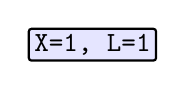
\begin{tikzpicture}[baseline=(a.base)]
				\node[draw=black,line width=0.8pt,fill=blue!10,rectangle,rounded corners=1pt,inner sep=2pt] (a) {\texttt{X=1, L=1}};
			\end{tikzpicture}
			$\to$
			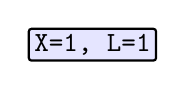
\begin{tikzpicture}[baseline=(b.base)]
				\node[draw=black,line width=0.8pt,fill=blue!10,rectangle,rounded corners=1pt,inner sep=2pt] (b) {\texttt{X=1, L=1}};
			\end{tikzpicture}
		} (state1);
		
		% Transition state1 -> state2: (X=0,L=0) -> (X=1,L=1)
		\draw[->] (state1) -- node[above] {%
			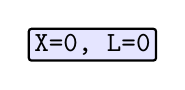
\begin{tikzpicture}[baseline=(a.base)]
				\node[draw=black,line width=0.8pt,fill=blue!10,rectangle,rounded corners=1pt,inner sep=2pt] (a) {\texttt{X=0, L=0}};
			\end{tikzpicture}
			$\to$
			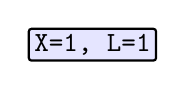
\begin{tikzpicture}[baseline=(b.base)]
				\node[draw=black,line width=0.8pt,fill=blue!10,rectangle,rounded corners=1pt,inner sep=2pt] (b) {\texttt{X=1, L=1}};
			\end{tikzpicture}
		} (state2);
		
		% Transition state2 -> state3: (X=0,L=0) -> (X=0,L=0)
		\draw[->] ([yshift=4pt]state2.east) to[out=50,in=180]
		node[above,sloped] {%
			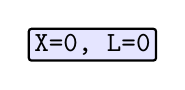
\begin{tikzpicture}[baseline=(a.base)]
				\node[draw=black,line width=0.8pt,fill=blue!10,rectangle,rounded corners=1pt,inner sep=2pt] (a) {\texttt{X=0, L=0}};
			\end{tikzpicture}
			$\to$
			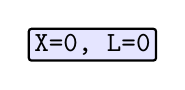
\begin{tikzpicture}[baseline=(b.base)]
				\node[draw=black,line width=0.8pt,fill=blue!10,rectangle,rounded corners=1pt,inner sep=2pt] (b) {\texttt{X=0, L=0}};
			\end{tikzpicture}
		} (state3.west);
		
		% Transition state2 -> state4: (X=1,L=1) -> (X=0,L=0)
		\draw[->] ([yshift=-16pt]state2.east) to[out=-50,in=180]
		node[below,sloped] {%
			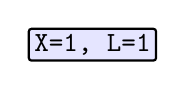
\begin{tikzpicture}[baseline=(a.base)]
				\node[draw=black,line width=0.8pt,fill=blue!10,rectangle,rounded corners=1pt,inner sep=2pt] (a) {\texttt{X=1, L=1}};
			\end{tikzpicture}
			$\to$
			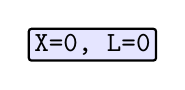
\begin{tikzpicture}[baseline=(b.base)]
				\node[draw=black,line width=0.8pt,fill=blue!10,rectangle,rounded corners=1pt,inner sep=2pt] (b) {\texttt{X=0, L=0}};
			\end{tikzpicture}
		} (state4.west);
		
		% To responses
		\draw[->] (state3) -- (resp0);
		\draw[->] (state4) -- (resp1);
		
	\end{tikzpicture}
	
	\caption{Network System for interleaving executions of the program in Listing~\ref{lst:MotivatingExample3Ser}.}
\label{fig:code3ExampleNS}
\end{figure}



%\begin{figure}[!htbp]
%	\centering
%	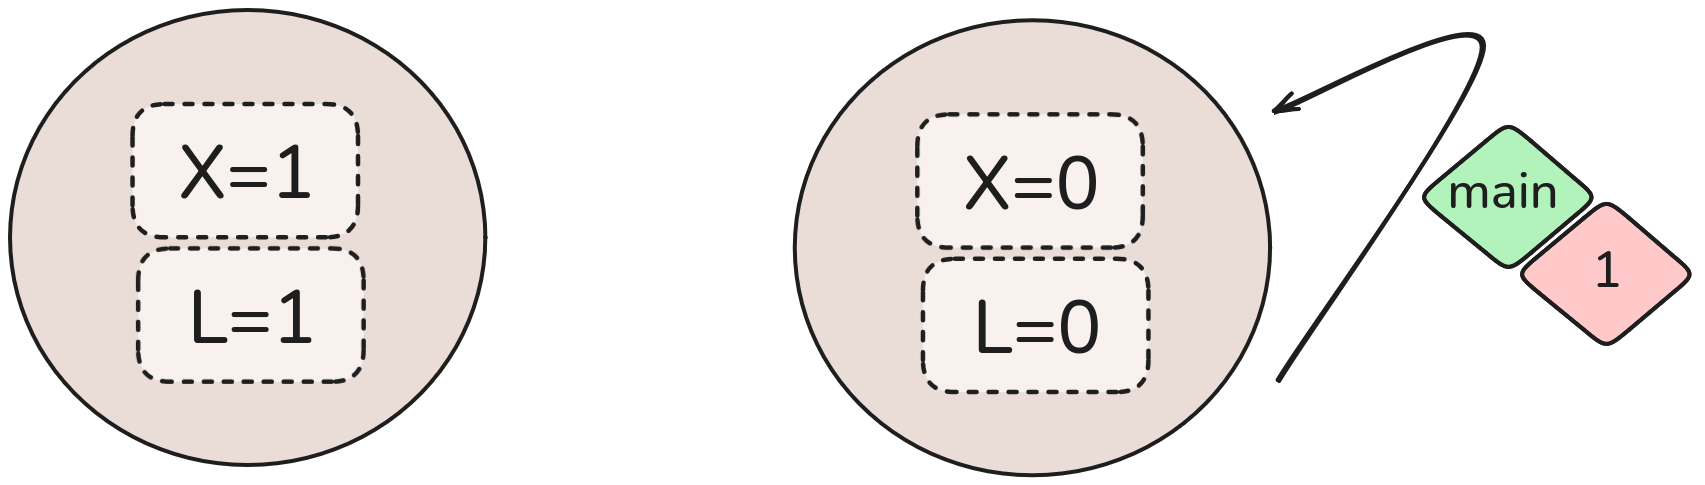
\includegraphics[width=0.4\textwidth]{plots/code_3_NFA.png}
%	\caption{NFA for serial executions of the program in Listing~\ref{lst:MotivatingExample3Ser}.}
%	\label{fig:code3ExampleNFA}
%\end{figure}


\begin{figure}  [!htbp]
	\centering
	% \includegraphics[width=0.48\textwidth,trim=0 0 0 0,clip]{plots/code_two_states_XL_NFA.pdf}
	
	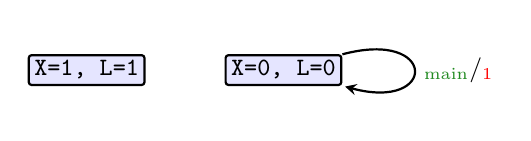
\begin{tikzpicture}[
		->,>=stealth,
		thick,
		node distance=2.5cm,
		state/.style={
			draw=black,
			line width=0.8pt,
			fill=blue!10,
			rectangle,
			rounded corners=1pt,
			inner sep=2pt,
			font=\small
		},
		every node/.style={font=\small}
		]
		% States
		\node[state] (X1L1) {\texttt{X=1, L=1}};
		\node[state, right of=X1L1] (X0L0) {\texttt{X=0, L=0}};
		
		% No edges to or from X=1, L=1 (isolated)
		
		% Self-loop on X=0, L=0 with main/1 (colored lozenge notation)
		\draw[->] (X0L0) edge[loop right]
		node[right] {${\color{ForestGreen}\blacklozenge_{\mathrm{main}}}/{\color{red}\blacklozenge_1}$} (X0L0);
	\end{tikzpicture}
	
	\caption{NFA for serial executions of the program in Listing~\ref{lst:MotivatingExample3Ser}.}
\label{fig:code3ExampleNFA}
\end{figure}




\begin{figure}[!htbp]
	\centering
	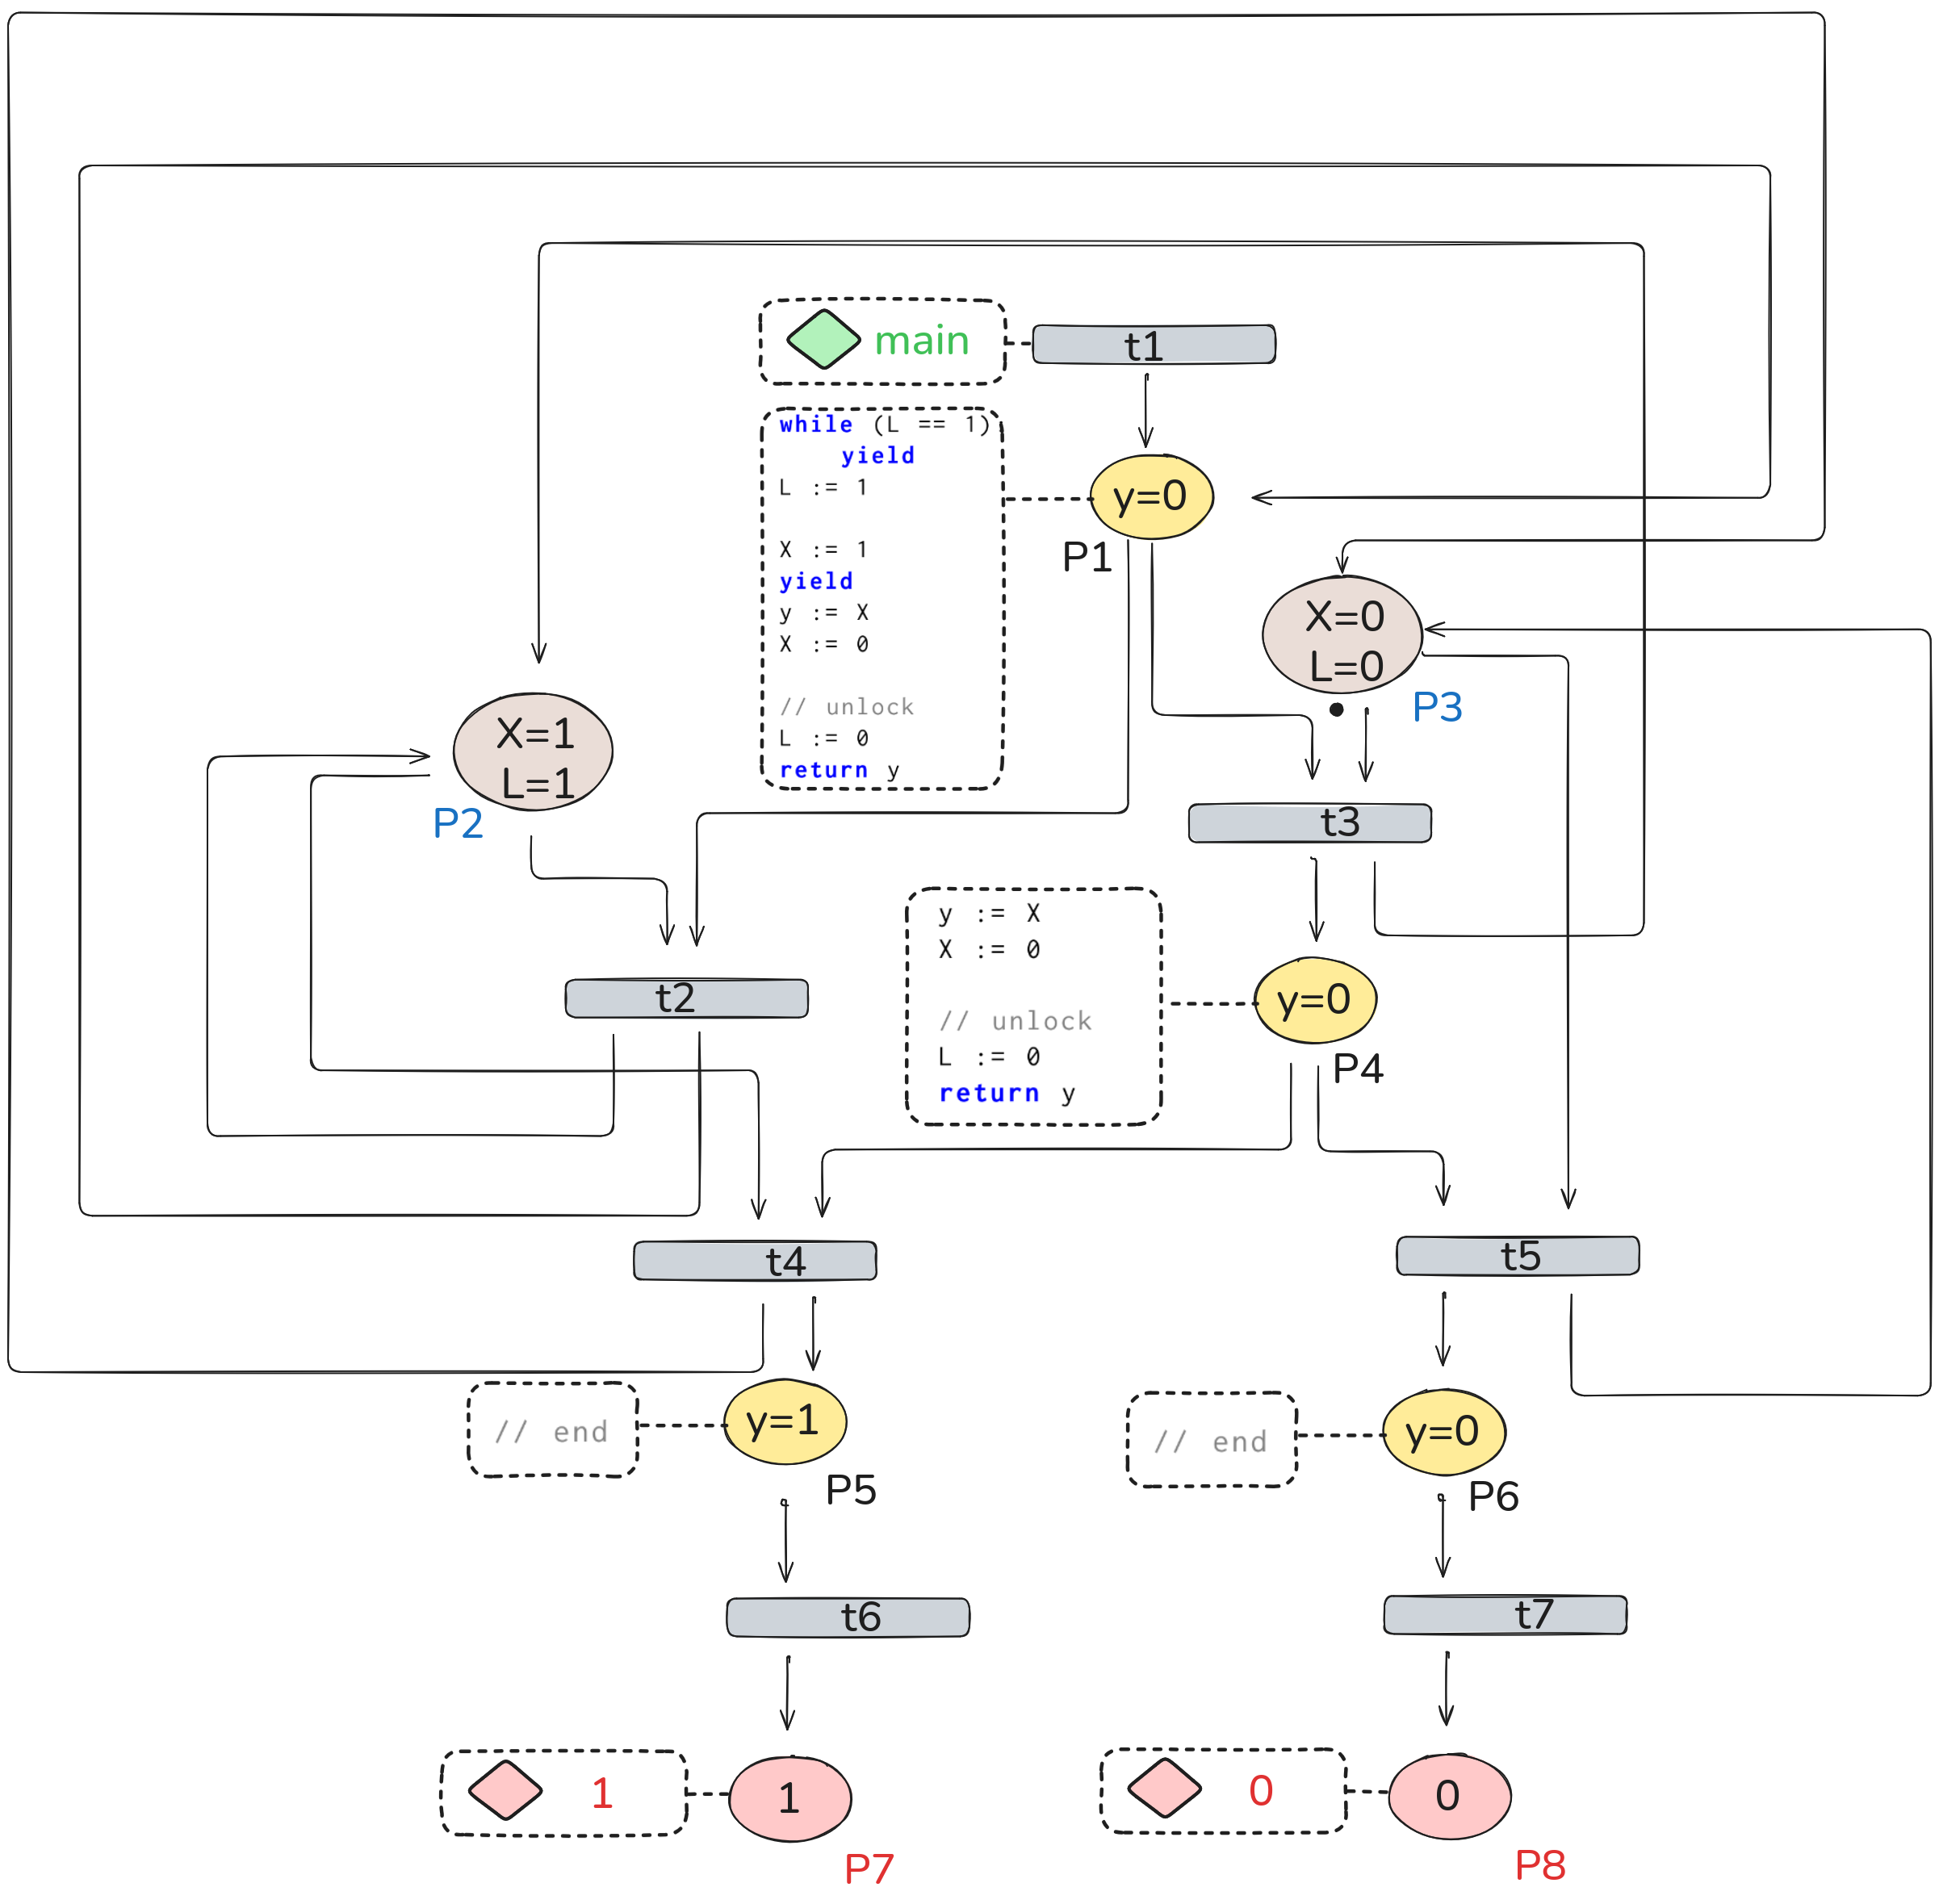
\includegraphics[width=0.8\textwidth]{plots/code_3_PN_with_annotation.png}
	\caption{Petri Net for interleaving executions of the program in Listing~\ref{lst:MotivatingExample3Ser}.}
	\label{fig:code3ExamplePN}
\end{figure}

%\newpage